\documentclass[border = 2mm]{standalone}
\usepackage[utf8]{inputenc}
\usepackage{tikz}
\usetikzlibrary{positioning, calc}

% Wiring of the outdoor station: every link is a cable with a connector
% (Grove, Grove to female jumpers, JST) or a wire held by a screw terminal.

\tikzset{
    module/.style={draw, thick, rounded corners=2pt, fill=#1, align=center,
        font=\sffamily\small, minimum height=1cm, minimum width=2.6cm},
    module/.default=gray!15,
    hub/.style={draw, thick, rounded corners=2pt, fill=gray!30, align=center,
        font=\sffamily\scriptsize, minimum height=0.9cm, minimum width=2.2cm},
    zone/.style={draw, dashed, thick, rounded corners=6pt},
    zonelabel/.style={font=\sffamily\bfseries\small, anchor=north west},
    port/.style={font=\sffamily\tiny, inner sep=1pt},
    wireI2c/.style={blue!70!black, very thick},
    wireSignal/.style={magenta!80!black, very thick},
    wirePower/.style={red!80!black, very thick},
    wireGround/.style={black, very thick},
    reserved/.style={gray, very thick, dashed},
    note/.style={font=\sffamily\scriptsize, align=center},
}

\begin{document}
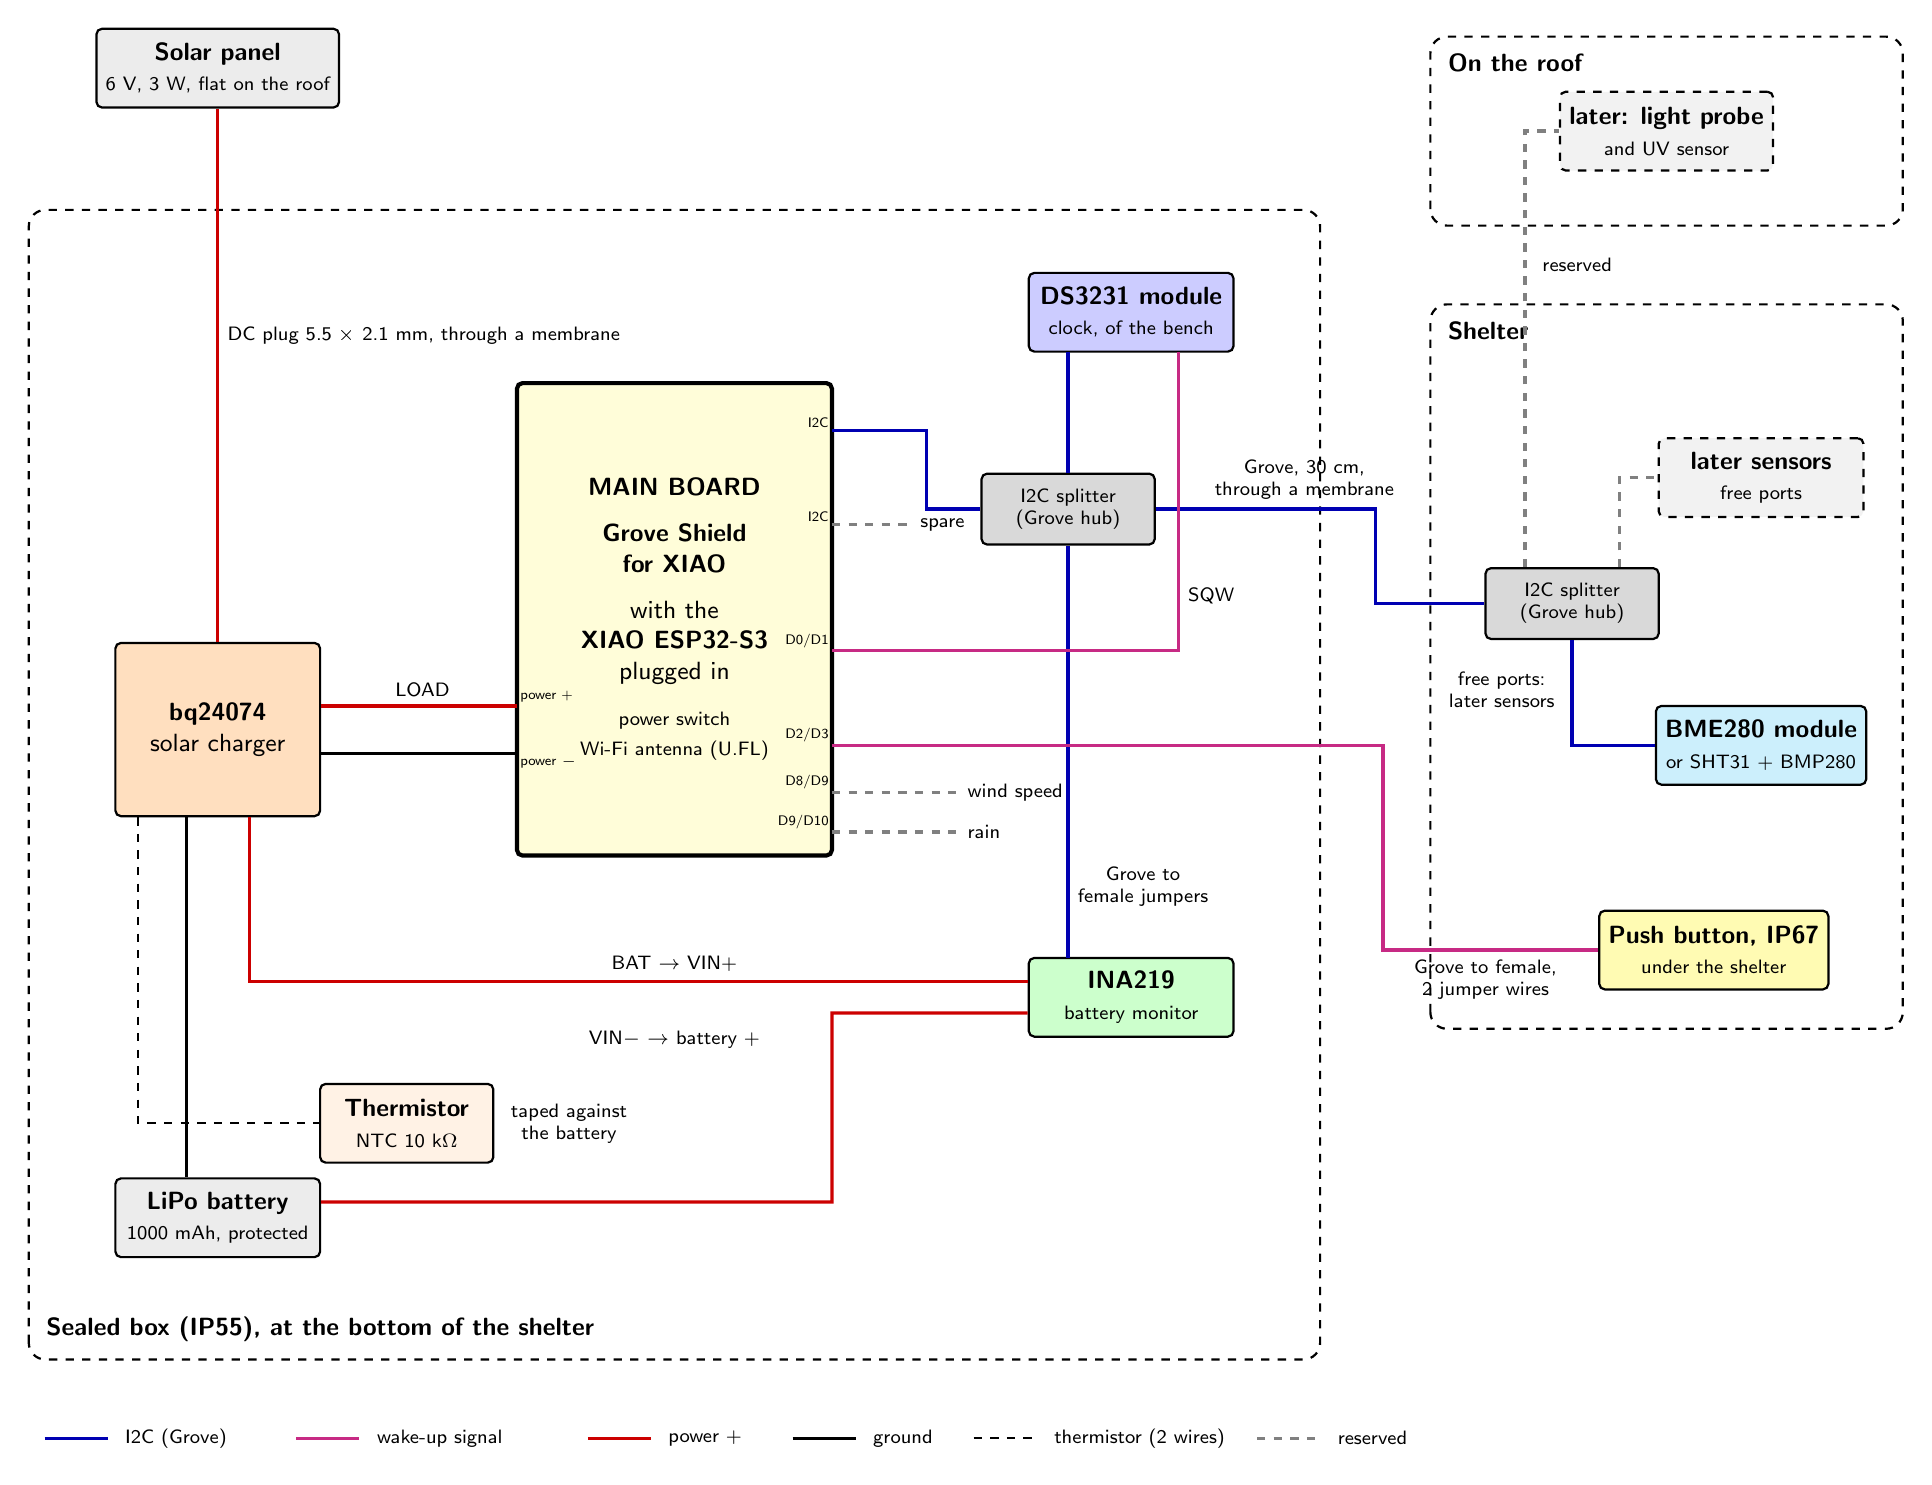
\begin{tikzpicture}

% ---------------------------------------------------------------- zones
\draw[zone] (-6.2,-6.4) rectangle (10.2,8.2);
\node[zonelabel, anchor=south west] at (-6.1,-6.3) {Sealed box (IP55), at the bottom of the shelter};

\draw[zone] (11.6,-2.2) rectangle (17.6,7.0);
\node[zonelabel] at (11.7,6.9) {Shelter};

\draw[zone] (11.6,8.0) rectangle (17.6,10.4);
\node[zonelabel] at (11.7,10.3) {On the roof};

% ---------------------------------------------------------------- modules
% The XIAO plugs into the female headers of the Grove Shield
\node[module=yellow!15, minimum width=4cm, minimum height=6cm, line width=1.5pt] (shield) at (2,3)
    {\textbf{MAIN BOARD}\\[2mm]\textbf{Grove Shield}\\\textbf{for XIAO}\\[2mm]
     with the\\\textbf{XIAO ESP32-S3}\\plugged in\\[2mm]
     \scriptsize power switch\\\scriptsize Wi-Fi antenna (U.FL)};

\node[hub] (hubA) at (7.0,4.4) {I2C splitter\\(Grove hub)};
\node[module=blue!20] (rtc) at (7.8,6.9) {\textbf{DS3231 module}\\\scriptsize clock, of the bench};
\node[module=green!20] (ina) at (7.8,-1.8) {\textbf{INA219}\\\scriptsize battery monitor};

\node[module=orange!25, minimum height=2.2cm] (charger) at (-3.8,1.6)
    {\textbf{bq24074}\\solar charger};
\node[module=gray!15] (battery) at (-3.8,-4.6) {\textbf{LiPo battery}\\\scriptsize 1000 mAh, protected};
\node[module=gray!15] (panel) at (-3.8,10.0) {\textbf{Solar panel}\\\scriptsize 6 V, 3 W, flat on the roof};

\node[hub] (hubB) at (13.4,3.2) {I2C splitter\\(Grove hub)};
\node[module=cyan!20] (sht) at (15.8,1.4) {\textbf{BME280 module}\\\scriptsize or SHT31 + BMP280};
\node[module=gray!10, dashed] (bmp) at (15.8,4.8) {\textbf{later sensors}\\\scriptsize free ports};
\node[module=yellow!30] (button) at (15.2,-1.2) {\textbf{Push button, IP67}\\\scriptsize under the shelter};
\node[module=gray!10, dashed] (probe) at (14.6,9.2) {\textbf{later: light probe}\\\scriptsize and UV sensor};

% ---------------------------------------------------------------- shield ports
\coordinate (i2cA) at (4,5.4);
\coordinate (i2cB) at (4,4.2);
\coordinate (pD0)  at (4,2.6);
\coordinate (pD2)  at (4,1.4);
\coordinate (pD8)  at (4,0.8);
\coordinate (pD9)  at (4,0.3);
\coordinate (bat)  at (0,1.9);
\coordinate (gnd)  at (0,1.3);
\node[port, anchor=south east] at (i2cA) {I2C};
\node[port, anchor=south east] at (i2cB) {I2C};
\node[port, anchor=south east] at (pD0)  {D0/D1};
\node[port, anchor=south east] at (pD2)  {D2/D3};
\node[port, anchor=south east] at (pD8)  {D8/D9};
\node[port, anchor=south east] at (pD9)  {D9/D10};
\node[port, anchor=south west] at (bat)  {power +};
\node[port, anchor=north west] at (gnd)  {power $-$};

% ---------------------------------------------------------------- I2C, in the box
% Grove port -> hub; the modules have pin headers: Grove to female jumpers
\draw[wireI2c] (i2cA) -- (5.2,5.4) |- (hubA.west);
\draw[wireI2c] (hubA.north) -- (7.0,6.4);
\draw[wireI2c] (hubA.south) -- (7.0,-1.3);
\node[note, right] at (7.0,-0.4) {Grove to\\female jumpers};
\draw[reserved] (i2cB) -- (5.0,4.2);
\node[note, right] at (5.0,4.2) {spare};

% ---------------------------------------------------------------- I2C, in the shelter
\draw[wireI2c] (hubA.east) -- (10.9,4.4) |- (hubB.west);
\node[note, above] at (10.0,4.4) {Grove, 30 cm,\\through a membrane};
\draw[wireI2c] (hubB.south) |- (sht.west);
\draw[reserved] ($(hubB.north)+(0.6,0)$) |- (bmp.west);
\draw[reserved] ($(hubB.north)+(-0.6,0)$) |- (probe.west);
\node[note, right] at (12.9,7.5) {reserved};
\node[note, left] at (13.3,2.1) {free ports:\\later sensors};

% ---------------------------------------------------------------- wake-up signals
% The alarm of the clock: its yellow lead (D0) on the SQW pin
\draw[wireSignal] (pD0) -- (8.4,2.6) -- (8.4,6.4);
\node[note, right] at (8.4,3.3) {SQW};
% The maintenance button closes D2 to ground while it is pressed
\draw[wireSignal] (pD2) -- (11.0,1.4) |- (button.west);
\node[note, below] at (12.3,-1.2) {Grove to female,\\2 jumper wires};

% ---------------------------------------------------------------- reserved
\draw[reserved] (pD8) -- (5.6,0.8);
\draw[reserved] (pD9) -- (5.6,0.3);
\node[note, right] at (5.6,0.8) {wind speed};
\node[note, right] at (5.6,0.3) {rain};

% ---------------------------------------------------------------- power
\draw[wirePower] (panel.south) -- (charger.north);
\node[note, right] at (-3.8,6.6) {DC plug 5.5 × 2.1 mm, through a membrane};

% LOAD output -> power bonding pad of the shield (its battery input)
\draw[wirePower] (charger.east |- bat) -- (bat);
\draw[wireGround] (charger.east |- gnd) -- (gnd);
\node[note, above] at (-1.2,1.9) {LOAD};

% BAT output -> INA219 -> battery: the INA219 measures what goes in and out
\draw[wirePower] ($(charger.south)+(0.4,0)$) |- ($(ina.west)+(0,0.2)$);
\node[note, above] at (2,-1.6) {BAT $\rightarrow$ VIN+};
\draw[wirePower] ($(ina.west)+(0,-0.2)$) -- (4.0,-2.0) |- ($(battery.east)+(0,0.2)$);
\node[note, below] at (2,-2.1) {VIN$-$ $\rightarrow$ battery +};
\draw[wireGround] ($(charger.south)+(-0.4,0)$) -- ($(battery.north)+(-0.4,0)$);

% Thermistor taped against the battery, wired to the charger only
% (its THERM pad and its ground)
\node[module=orange!10, minimum width=2.2cm] (ntc) at (-1.4,-3.4) {\textbf{Thermistor}\\\scriptsize NTC 10 k$\Omega$};
\draw[thick, dashed] ($(charger.south west)+(0.3,0)$) |- (ntc.west);
\node[note, right] at (-0.2,-3.4) {taped against\\the battery};

% ---------------------------------------------------------------- legend
\begin{scope}[shift={(-6,-7.4)}]
    \draw[wireI2c] (0,0) -- (0.8,0); \node[note, right] at (0.9,0) {I2C (Grove)};
    \draw[wireSignal] (3.2,0) -- (4.0,0); \node[note, right] at (4.1,0) {wake-up signal};
    \draw[wirePower] (6.9,0) -- (7.7,0); \node[note, right] at (7.8,0) {power +};
    \draw[wireGround] (9.5,0) -- (10.3,0); \node[note, right] at (10.4,0) {ground};
    \draw[thick, dashed] (11.8,0) -- (12.6,0); \node[note, right] at (12.7,0) {thermistor (2 wires)};
    \draw[reserved] (15.4,0) -- (16.2,0); \node[note, right] at (16.3,0) {reserved};
\end{scope}

\end{tikzpicture}
\end{document}
